\documentclass{beamer}

\usepackage{default}
\usepackage{graphicx}
\usepackage{amsmath}

\usetheme{HUmetrics}

\title[A Statistical Variant of the Inductive Miner]{A Statistical Variant of the Inductive Miner}
\author[Kurzname]{Martin Bauer}
\institute{Institut für Informatik\\Humboldt-Universität zu Berlin}
\date{16.6.2017}

\begin{document}

\titlepage
\begin{frame}
\centering
\frametitle{Contents of this presentation}
\begin{itemize}
\item Process Mining
\item Incremental Log Analysis
\item the Statistical Inductive Miner infrequent
\item Discussion
\end{itemize}
\end{frame}

\begin{frame}
\frametitle{Process Mining}
\begin{columns}
\column{0.5\linewidth}
\centering
\begin{tabular}{l|c|l}
 user id & activity & timestamp\\
 \hline
 3456 & A & 03-07-2016\\
 3456 & B & 03-07-2016\\
 4788 & A & 04-07-2016\\
 3456 & C & 04-07-2016\\
 4788 & D & 04-07-2016\\
 \end{tabular}
 \column{0.5\linewidth}
 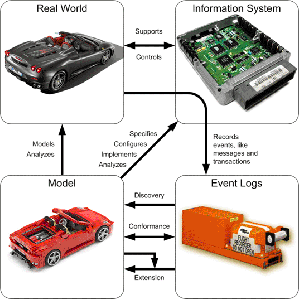
\includegraphics[width=0.9\linewidth]{processmining.png}
\end{columns}
\end{frame}

\begin{frame}
\frametitle{Process Discovery}
\begin{columns}
\column{0.3\linewidth}
\begin{tabular}{l|c}
 user id & activity\\
 \hline
 1 & A\\
  1 & B\\
 1 & E\\
 2 & B\\
  2 & A\\
 2 & C\\
 3 & B\\
  3 & A\\
 3 & C\\
 3 & D\\
 3 & C\\
 \end{tabular}
\column{0.7\linewidth}
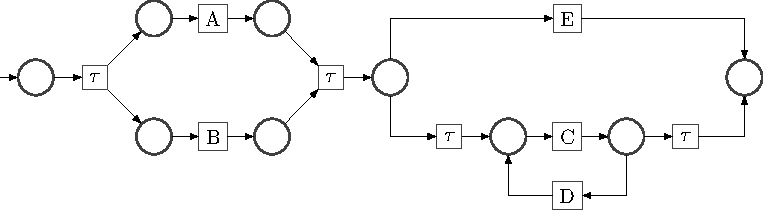
\includegraphics[width=0.8\linewidth]{img/petri-net.pdf}
\end{columns}
\end{frame}

%\begin{frame}
%\frametitle{Block-structured Models}
%\centering
%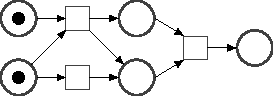
\includegraphics[width=0.4\linewidth]{img/petri_deadlock.pdf}\vspace{0.3cm}
%\hline\vspace{0.3cm}
%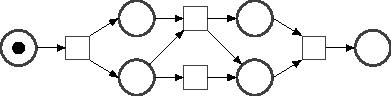
\includegraphics[width=0.5\linewidth]{img/wfnet.pdf}\\
%\vspace{0.3cm}\hline\vspace{0.3cm}
%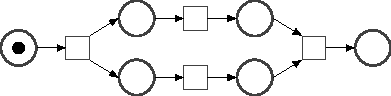
\includegraphics[width=0.5\linewidth]{img/bswfnet.pdf}
%\end{frame}

\begin{frame}
\frametitle{Inductive Miner - Conversion to df-Graph}
\begin{columns}
\column{0.3\linewidth}
\centering
\begin{tabular}{l|c}
 user id & activity\\
 \hline
 1 & A\\
  1 & B\\
 1 & E\\
 2 & B\\
  2 & A\\
 2 & C\\
 3 & B\\
  3 & A\\
 3 & C\\
 3 & D\\
 3 & C\\
 \end{tabular}
\column{0.7\linewidth}
\centering
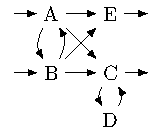
\includegraphics[width=0.4\linewidth]{img/dfgraphExample.pdf}
\end{columns}
\end{frame}

\begin{frame}
\frametitle{Inductive Miner - Detecting Cuts}
\begin{columns}
\column{0.5\linewidth}
\centering
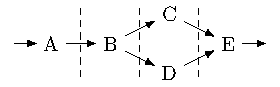
\includegraphics[width=0.8\linewidth]{img/seq_cut.pdf}\\
\vspace{1cm}
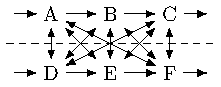
\includegraphics[width=0.7\linewidth]{img/and_cut.pdf}
\column{0.5\linewidth}
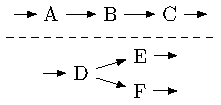
\includegraphics[width=0.7\linewidth]{img/xor_cut.pdf}\\
\vspace{1cm}
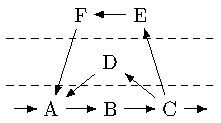
\includegraphics[width=0.7\linewidth]{img/loop_cut.pdf}
\end{columns}
\end{frame}

\begin{frame}
\frametitle{Inductive Miner - Building a Process Tree}
\begin{columns}
\column{0.5\linewidth}
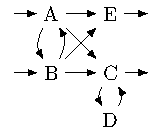
\includegraphics[width=0.8\linewidth]{img/dfgraphExample.pdf}
\column{0.5\linewidth}
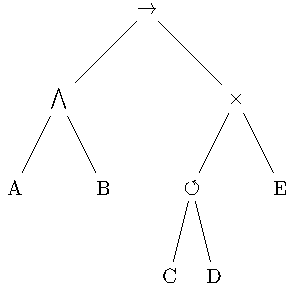
\includegraphics[width=0.8\linewidth]{img/xor_tree_final.pdf}
\end{columns}
\end{frame}

\begin{frame}
\frametitle{Inductive Miner infrequent - Filtering out Noise}
\begin{columns}
\column{0.5\linewidth}
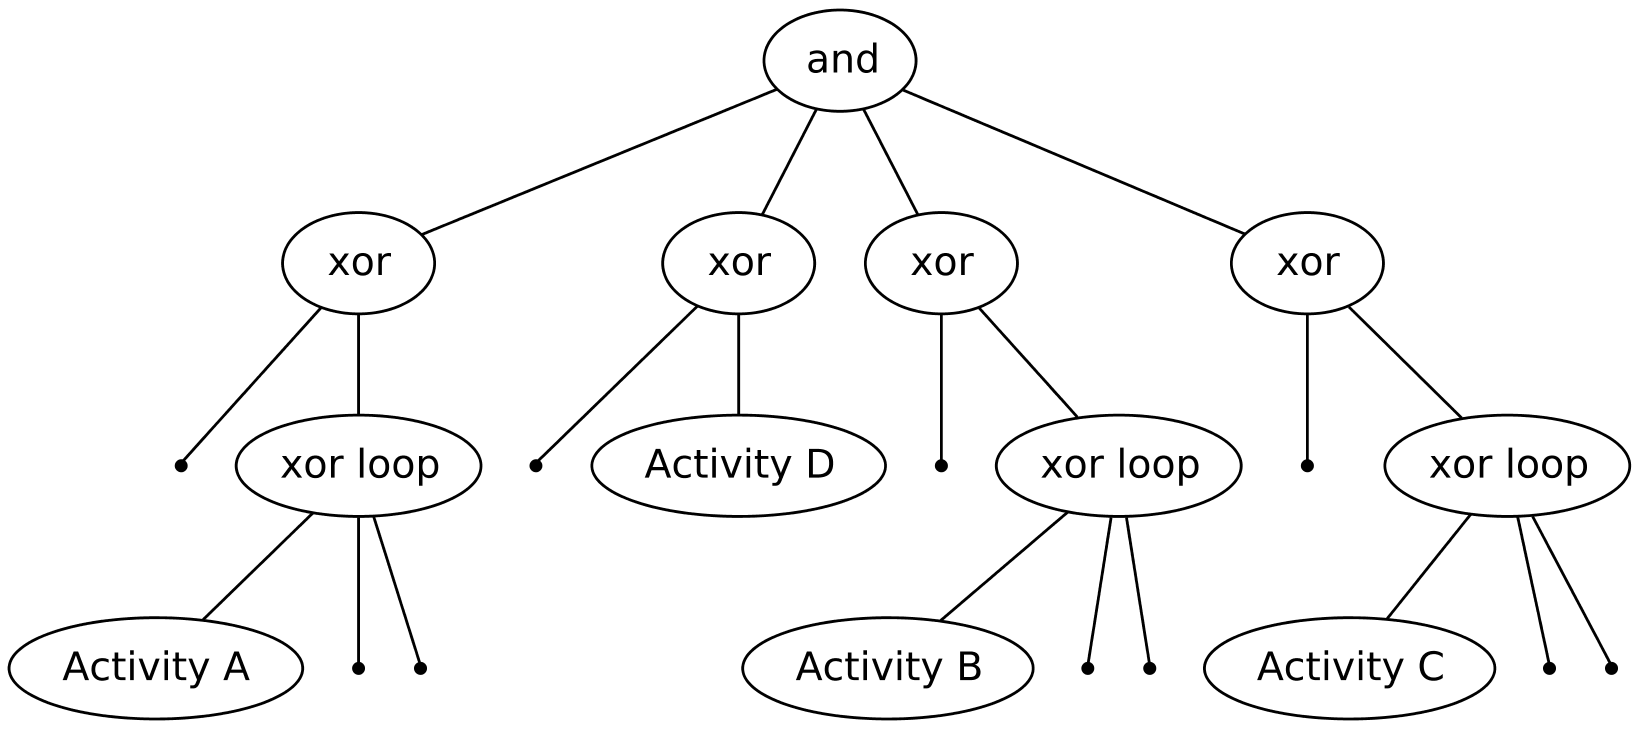
\includegraphics[width=0.8\linewidth]{img/noise.png}
\column{0.5\linewidth}
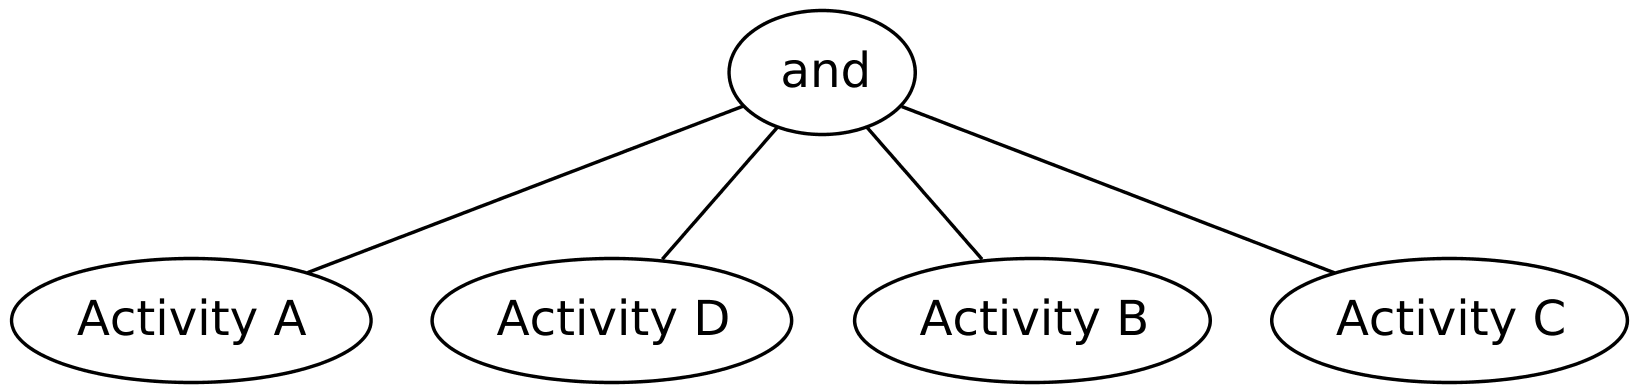
\includegraphics[width=0.89\linewidth]{img/noiseless.png}
\end{columns}
\end{frame}

\begin{frame}
\frametitle{Incremental Process Discovery - Redundancy of Logs}
\begin{itemize}
\item A,B,C,D - 500
\item A,B,E - 400
\item A,G - 20
\end{itemize}
How likely are we to see new information in the next N Traces?\\
\begin{align*}
Bin(N,k)=\binom{N}{k}\cdot p^k\cdot (1-p)^{N-k}
\end{align*}
\end{frame}

\begin{frame}
\frametitle{Delta-Completeness}
\centering
\large
"A Log is $\delta$-complete, if the probability p of seeing new information in the next trace is smaller than $\delta$"
\end{frame}

\begin{frame}
\frametitle{Incremental Process Discovery - Estimating p}
\begin{align*}
[\frac{1}{1+\frac{z^2}{N}}\cdot(p^{\hat{}}+\frac{z^2}{2N}-\sqrt{\frac{p^{\hat{}}\cdot(1-p^{\hat{}})}{N}+\frac{z}{4N^2}}),\\\frac{1}{1+\frac{z^2}{N}}\cdot(p^{\hat{}}+\frac{z^2}{2N}+\sqrt{\frac{p^{\hat{}}\cdot(1-p^{\hat{}})}{N}+\frac{z}{4N^2}})]
\end{align*}\\
Assuming $p^{\hat{}}=0$ gives
\begin{align*}
\frac{1}{1+\frac{z^2}{N}}\cdot(\frac{z^2}{2\cdot N}+\sqrt{\frac{z}{4\cdot N^2}})
\end{align*}

Increase N until upper bound is smaller than $\delta$\\
\end{frame}

\begin{frame}
\frametitle{Content of the Thesis}
\begin{itemize}
\item Apply the Incremental Process Discovery Procedure to Inductive Miner infrequent using model correctness and approximated average cycle time as quality criteria
\item Evaluate the algorithm on runtime properties and on factors that influence it's effiency
\end{itemize}
\end{frame}

\begin{frame}
\frametitle{Model Correctness}
\begin{columns}
\column{0.5\linewidth}
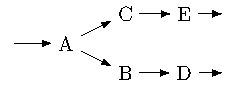
\includegraphics[width=0.8\linewidth]{img/dfgraph_before_trace.pdf}
\column{0.5\linewidth}
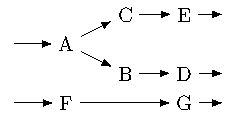
\includegraphics[width=0.8\linewidth]{img/dfgraph_added_trace.pdf}
\end{columns}\vspace{1cm}
A trace may add events, edges, starting- or ending nodes - if it does, it contains new information
\end{frame}

\begin{frame}
\frametitle{Cycle Time Correctness}
Trace-based and Event-based Cycle times
\begin{itemize}
\item A(5s), B(10s), C(5s)
\item A,B,C (20s)
\end{itemize}
\vspace{1cm}
Iterative Estimation of cycle time is converging towards correct cycle time:
\begin{align*}
\forall \epsilon\geq0 \exists 0<N<\max(|t|) \forall N\leq t_n,t_m <\max(|t|): d(cycle time_n, cycle time_m)<\epsilon
\end{align*}
given $\epsilon$, if trace changes cycle time more than $\epsilon$ assume new information
\end{frame}

\begin{frame}
\frametitle{The Algorithm}
\begin{center}
  \makebox[\textwidth]{\includegraphics[width=\paperwidth]{{algorithm.png}}}
\end{center}
\end{frame}

\begin{frame}
\frametitle{Evaluation - Runtime}
\begin{columns}
\column{0.5\linewidth}
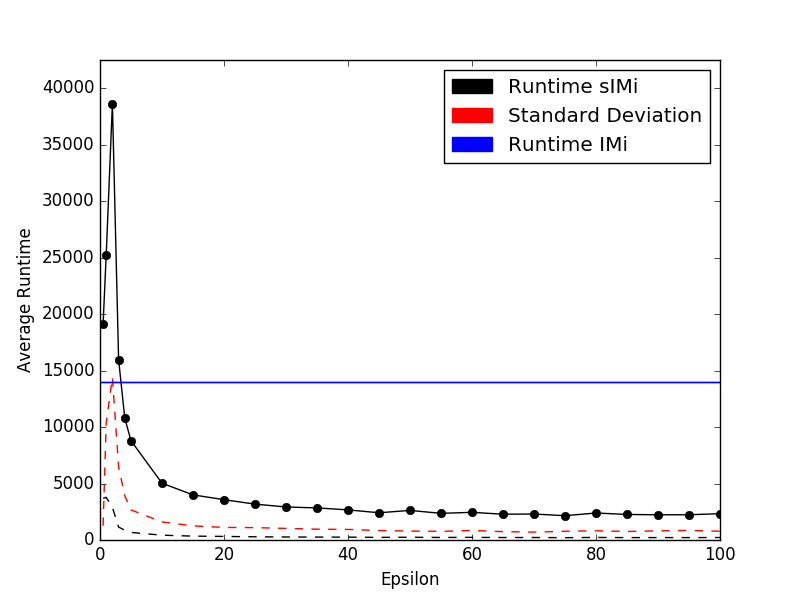
\includegraphics[width=0.95\linewidth]{data/BPI2014/BPI2014_lax_threshold_timeAllData.png}
\column{0.5\linewidth}
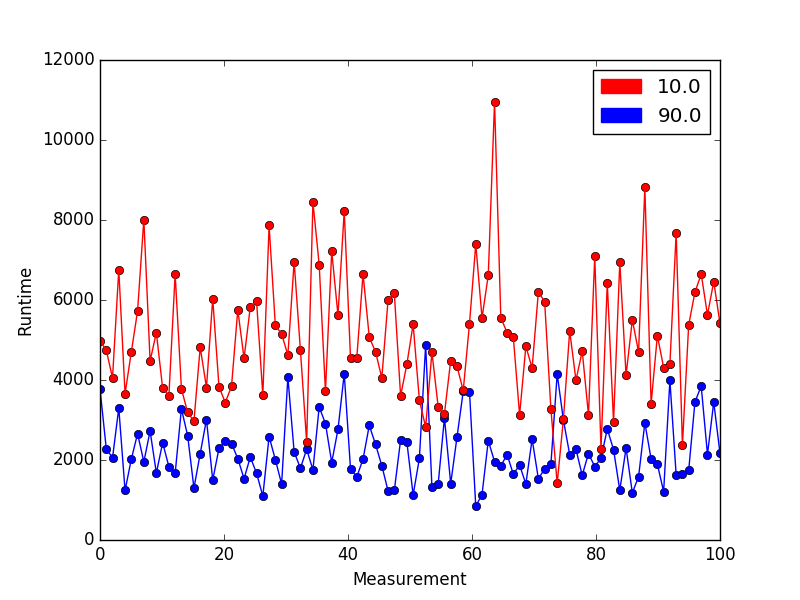
\includegraphics[width=0.95\linewidth]{data/BPI2014/lax_10_90_runtime.png}
\end{columns}
\end{frame}

\begin{frame}
\frametitle{Evaluation - Traces}
\centering
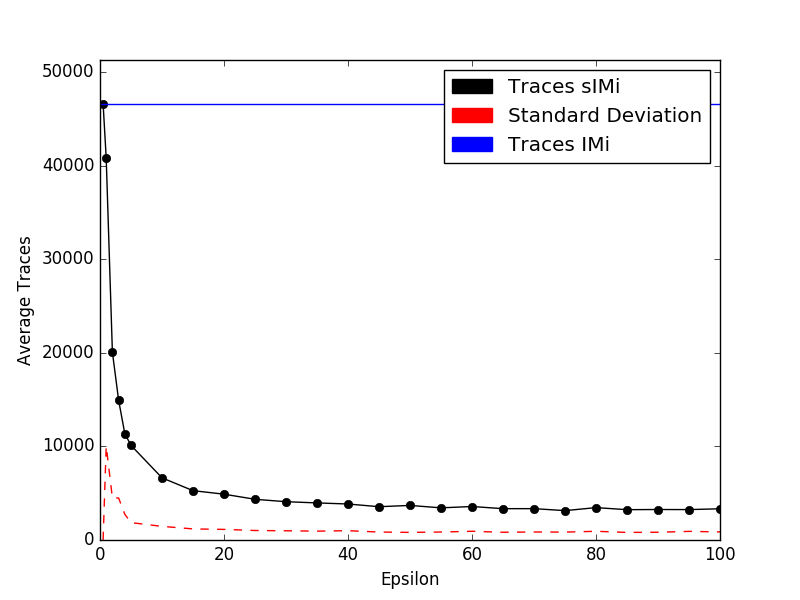
\includegraphics[width=0.5\linewidth]{data/BPI2014/BPI2014_lax_threshold_traces.png}
\end{frame}

\begin{frame}
\frametitle{Evaluation - Memory}
\centering
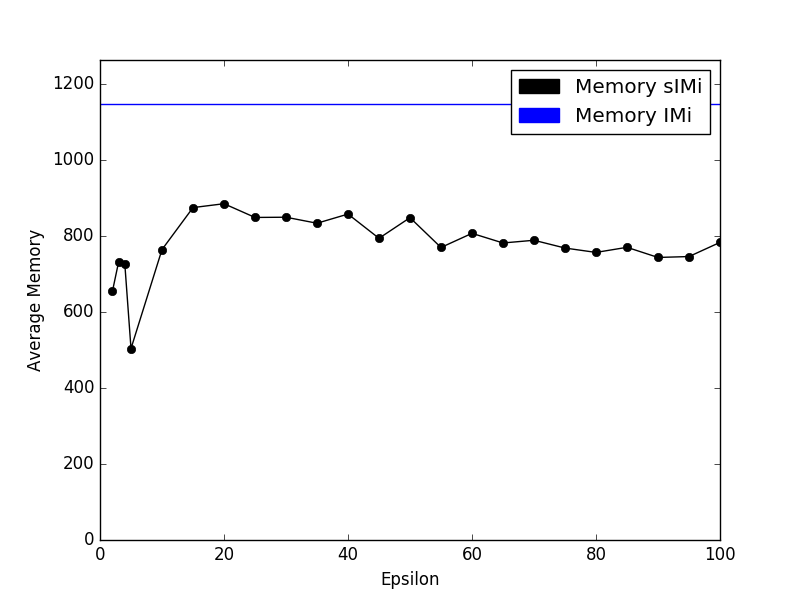
\includegraphics[width=0.5\linewidth]{data/BPI2014/BPI2014_lax_threshold_memory.png}
\end{frame}

\begin{frame}
\frametitle{Evaluation - what runtime approximation is better?}
\begin{columns}
\column{0.5\linewidth}
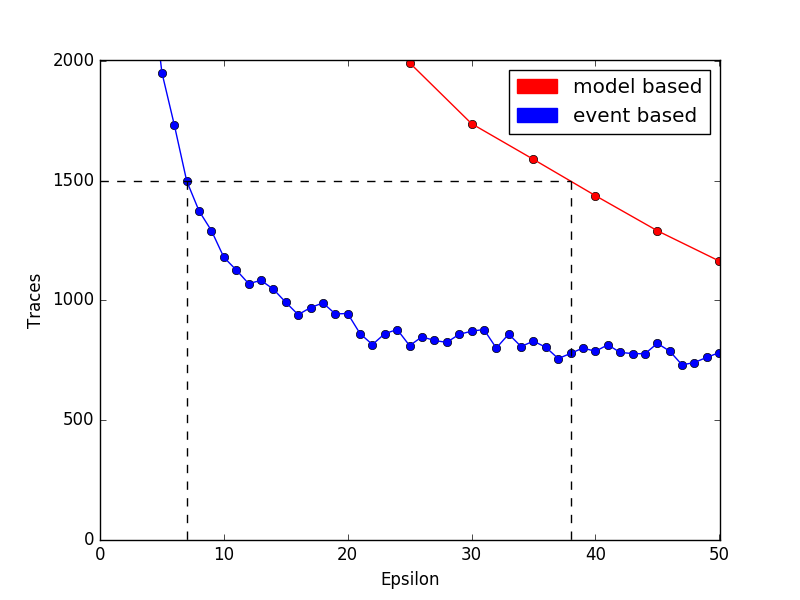
\includegraphics[width=0.95\linewidth]{data/lax_vs_strict_traces_epsilon_zoomed.png}
\column{0.5\linewidth}
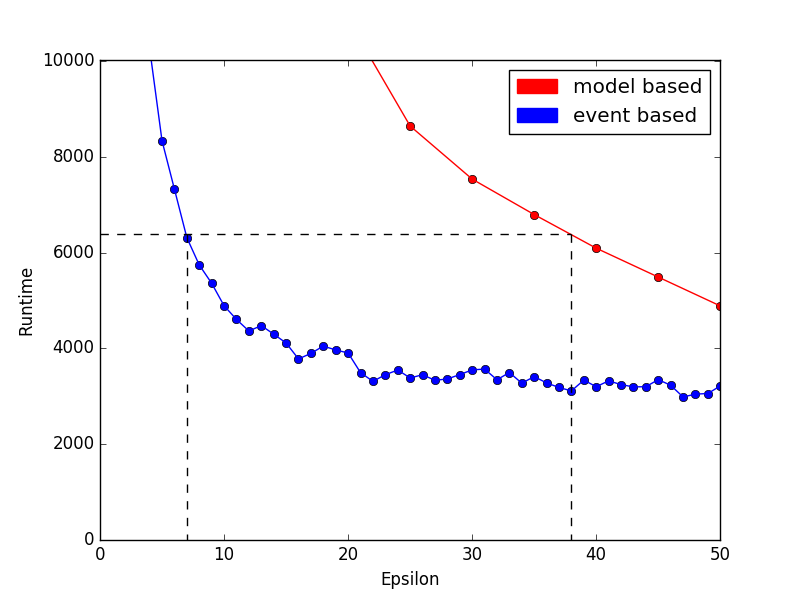
\includegraphics[width=0.95\linewidth]{data/kax_vs_strict_runtime_zoomed.png}
\end{columns}
\end{frame}

\begin{frame}
\frametitle{Evaluation - Fitness}
\centering
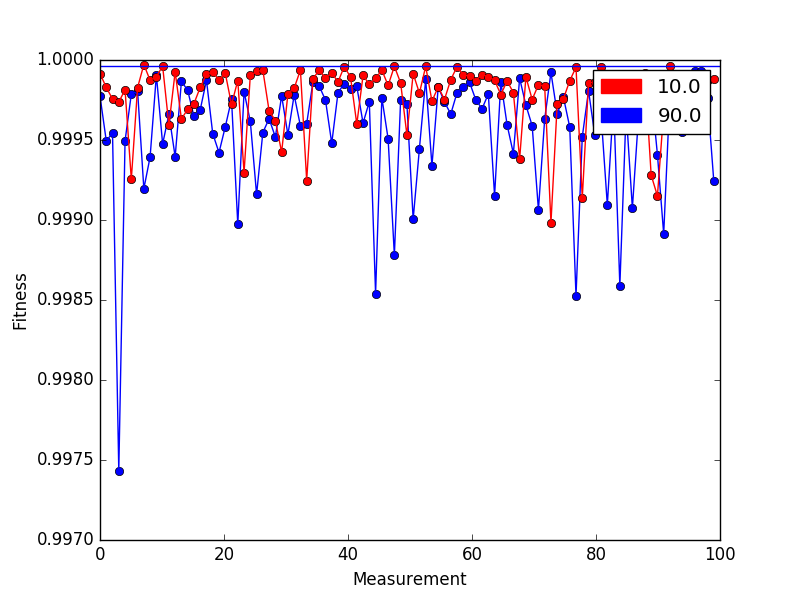
\includegraphics[width=0.5\linewidth]{data/BPI2014/lax_10_90_fitness.png}
\end{frame}

\begin{frame}
\frametitle{Log properties - Noise and Cycle Time Deviations}
\centering
\begin{columns}
\column{0.5\linewidth}
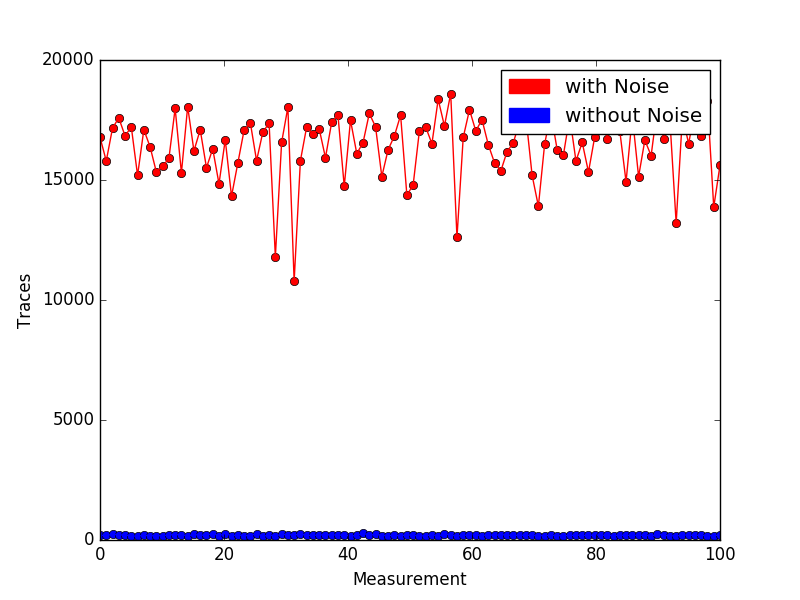
\includegraphics[width=0.95\linewidth]{img/Noise_Noiseless.png}
\column{0.5\linewidth}
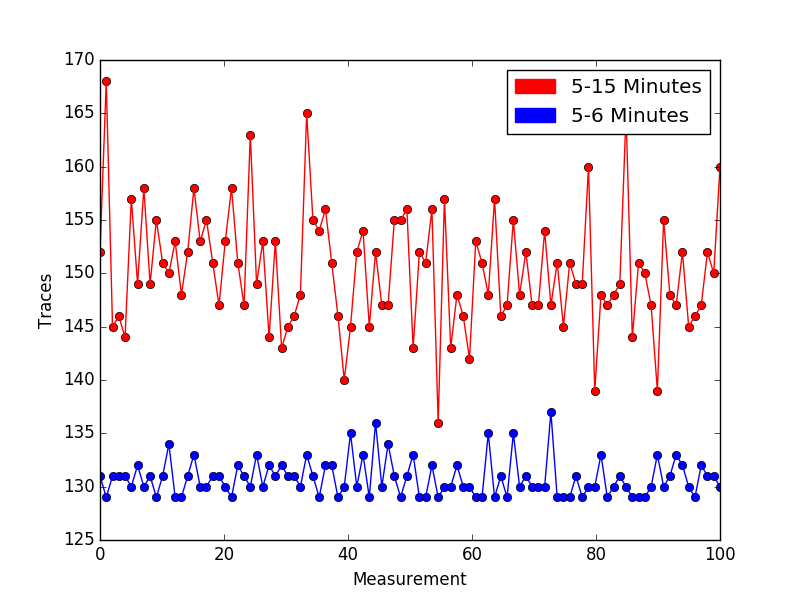
\includegraphics[width=0.95\linewidth]{img/high_vs_low_deviation.png}
\end{columns}
\end{frame}

\begin{frame}
\frametitle{Control flow structures}
\begin{columns}
\column{0.33\linewidth}
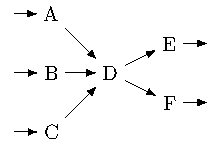
\includegraphics[width=0.9\linewidth]{img/sequence_xor_event_xor.pdf}
\column{0.33\linewidth}
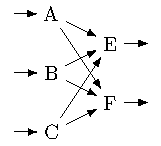
\includegraphics[width=0.9\linewidth]{img/sequence_xor_xor.pdf}
\column{0.33\linewidth}
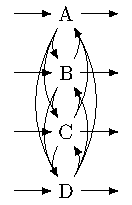
\includegraphics[width=0.6\linewidth]{img/and.pdf}
\end{columns}
AND and sequential complex blocks (AND, XOR) influence runtime the most
\end{frame}

\begin{frame}
\frametitle{Conclusion}
\begin{itemize}
\item sIMi outperforms IMi an almost all cases
\item the algorithmic framework is extensible
\item no fitness loss
\end{itemize}
\begin{itemize}
\item bad $\epsilon$ increase runtime by a lot
\item random nature of trace picking (can be adjusted easily)
\end{itemize}
\end{frame}

\begin{frame}
\Huge
\centering
Thank you!\\
Any questions?
\end{frame}
\end{document}
